A mesh network can use a wide variety of protocols, to manage the route data is transferred.
In networking, a protocol is a special set of rules and standards for how nodes would interacts with each other.
A well known protocols could be TCP/IP(Transmission Control Protocol/Internet Protocol), which today are used to communicate between almost anything with a internet connection.
The mesh network we are looking at is a radio based network, and therefore some more relevant protocols will be examined. 
A few excising protocols will be presented in this section.

\subsection{Time division multiple access}
Time division multiple access(TDMA) is protocol that divides a single channel into smaller time slots.
Each time slot transmits one byte or a segment of a signal, in a sequential serial data format.
Each slot is active of a small amount of time, before the next slot in the queue get time to transmit.

TDMA is as an example used in the T1 telecommunication transmission system.
Each T1 channels carry up to 24 voice telephone connections.
Where each connection covers 300 Hz to 3000Hz and is digitized at an 8-kHz rate, which is two times the highest frequency component needed to retain all the analog content.
\begin{figure}[!h]
	\centering
	\makebox[\textwidth][c]{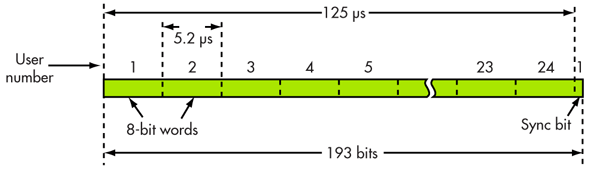
\includegraphics[width=1\textwidth]{figures/TDMA.png}}
	\caption{Illustration of the TDMA protocol}
	\label{fig:TDMAfigure}
\end{figure}

On \figref{TDMAfigure} it is seen how the channel, for T1, is split up into 24 smaller pieces.
Each time slot is accountant for a user using a voice channel, to talk to some other user.
Each time slot is of the size 8-bit, the user is unaware of this small data size, and that other are using the same channel, because the shift between each time slot happens so fast.
This gives the illusion of each user talking with no interruptions, even though each user only is assigned 1/24 of the total bandwidth.
A single bit is used to synchronization.
The TDMA system can maximum achieved a data rate of 1.544 Mbit/second.\cite{TDMA}

TDMA can be used for any system that require several device to use the same channel, without interfering with each other.


%\subsection{Radio Link Protocol}
%Radio Link protocol(RLP) is a automatic repeat request(ARQ)\footnote{An error-control method for data transmission that uses acknowledgements and timeouts} fragmentation protocol used over a wireless air interface.
%Most air interface protocols have a packet loss of up to 1\% which is intolerable when handling sensitive data.
%RLP detects losses in packets and with a retransmission tries to bring down the losses.
%The retransmission can bring the loss down to 0.1\% to 0.0001\%.
%This loss rate is more tolerable when handling sensitive and precise data.

%RPL cannot request a certain payload size from the air interface, the air interface scheduler instead determines the packet size, based on changing channel conditions constantly.
%Most of the other fragmentation protocols, such as 802.11b\footnote{An wireless networking specification} and IP, determine a payload of a certain size by the upper layers, and call upon the MAC.
%These protocols are not as flexible as RLP, and sometime fail transition during small fades in a wireless environment.\cite{MobileComm}

%RLP is used to make a more fail-safe environment for the transmitted data, and to ensure nothing is lost on the way.
%The Radio Link Protocol is typically used in cellular transmission.

\subsection{Dynamic Source Routing protocol}
The Dynamic Source Routing protocol (DSR) is a simple routing protocol designed specifically for use in multi-hop wireless ad hoc networks.
With DSR the network is completely self-organizing and self-configuring, requiring no administration or existing network structure.
The nodes in the network work together to forward packets to desternations that can be outside of the senders transmission range.
As nodes can be added and removed ad hoc, the protocol automatically determine and maintain the routing of the packets though out the network.
Since the number or sequence of nodes needed to reach any destination may change at any time, the resulting network topology may be quite rapidly changing.
DSR is created to create a very low overhead yet being able to react quickly to change in the network environment.
The protocol provides a highly reactive service to ensure successful delivery of data packets where node may be moving around, or other changes in the network occur. 

The DSR protocol is composed of two main mechanisms that allow the discovery and maintenance of the routes in the network.

- Route Discovery is the mechanism by which a node S wishing to send a packet to a destination node D obtains a source route to D.
Route Discovery is used only when S attempts to send a packet to D and does not already know a route to D.

- Route Maintenance is the mechanism by which node S is able to detect, while using a source route to D, if the network topology has changed such that it can no longer use its route to D 
because a link along the route no longer works.
When Route Maintenance indicates a source route is broken, S can attempt to use any other route it happens to know to D, or it can invoke Route Discovery again to find a new route for subsequent packets to D.
Route Maintenance for this route is used only when S is actually sending packets to D.

DSR is a source routing protocol where packets carries a header, a ordered list of nodes to determine the route.
This explicit use of routing allows the sender to select and control the route for the packets it sends.
Source routing allow for load balancing, since the sender can create different routes out though the network, avoiding "heavy traffic".
It is also guarantee that the routes used are loop-free, since a generated route never use the same node twice.
By including this source route in the header of each packet, other nodes forwarding or overhearing any of these packets can easily cache this information for future use.\cite{DSR}

\subsection{Ad hoc On-Demand Distance Vector Routing}
Ad hoc On Demand Distance Vector(AODV) routing algorithm is a routing protocol designed for ad hoc networks. 
It is an on demand algorithm, meaning that it builds routes between nodes only as desired by source nodes.\cite{AOVD1}

AODV is a network where only the local nodes around a newly added node, is affected by the addition.
If a link between nodes is broken, and it does not affect an ongoing transmission, no global notification occurs.
This leads to a network where new nodes easily can be added and removed without overhead on the entire network.
The transmission  route in AODV is managed so, that only nodes in the direct route is active, which reduce the need for route maintenance and reduce idle nodes.
The protocol can determine multiple routes between a source and a destination, but only a single one is implemented.
The route is not necessarily the shortest.

A downside to AODV is that if a single route breaks, due to a defect node, it is not possible to know whether other routes exists.
But if a route breaks, the protocol discovers a new route, if possible, as and when necessary.

When a node is ordered to send a packet to a specified destination, it checks its routing table to determine if it has a current route to the destination.
If there already exist a node, the packet will be delivered to the next node in the route, repeating until it arrives at the correct location.
If there does not exist a route, the node will initiates a route discovery process.

A route discovery process begins with the source creating a Route Request (RREQ) packet.
The packet contains the sources node's unique ID and IP, and the destination node's unique ID and IP.
The packet is then transmitted out from the source to it's neighbours.
The unique ID of each node is then stored in the packet, to ensure the same node is not transmitting more than once.
The destination ID is to ensure it knows when the destination node is reached.
A simple AODV network can be seen on \figref{AODVfigure}, where S and D represent the source and destination. It is visualized how the route discovery is invoked using the RREQ packet.\cite{AOVD2}

\begin{figure}[!h]
	\centering
	\makebox[\textwidth][c]{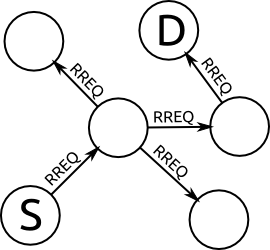
\includegraphics[width=0.4\textwidth]{figures/AODV.png}}
	\caption{Illustration of the AODV route discovery}
	\label{fig:AODVfigure}
\end{figure}

\subsection{Better approach to mobile ad-hoc networking}
Better approach to mobile ad-hoc networking (B.A.T.M.A.N) is a routing protocol for multi-hop ad-hoc mesh networks. 
B.A.T.M.A.N is said to solve some of the more typical problems with the classical routing protocols, which is not well suited for wireless ad-hoc networks.
Some of the problems is, such networks  are unstructured, are based on an inherently unreliable medium and dynamically change their topology.

When using the B.A.T.M.A.N algorithm, the approach is to divide the knowledge about the most reasonable path between nodes in a network to all of the participating nodes.
Each node in the network only account for the best path to all other nodes in the system.
This results in, the need for a global knowledge about local topology changes becomes unnecessary.
In addition, does B.A.T.M.A.N have an event-based, but timeless, flooding mechanism that prevents the occurrence of loops and limits the amount of topology messages flooding the network.
The protocol is designed to handle network where links between nodes are not always reliable.\cite{BATMAN}

\subsection{Protocol comparison}
Below is a comparison table with the protocol discuses in this chapter. Her skal skrives et eller andet.

\begin{table}[C]
\centering
\caption{Protocol comparison}
\label{my-label}
\begin{tabular}{|l|c|c|c|c|c|c|}
\hline
            & Ad hoc & Rute metrics                                                                     & \begin{tabular}[c]{@{}c@{}}Loop \\ Free\end{tabular} & \begin{tabular}[c]{@{}c@{}}Load \\ balancing\end{tabular} & Reliability & Thoughput                                                                    \\ \cline{1-1}
\rowcolor[HTML]{EFEFEF} 
TDMA        & Yes    & \begin{tabular}[c]{@{}c@{}}Routes ensuring\\  guaranteed bandwidth\end{tabular} & Yes                                                  & Yes                                                       & High        & \begin{tabular}[c]{@{}c@{}}Decreases as more \\ nodes are added\end{tabular} \\
DSR         & Yes    & Source routing                                                                   & Yes                                                  & No                                                        & High        & \begin{tabular}[c]{@{}c@{}}Decreases as more\\  nodes are added\end{tabular} \\
\rowcolor[HTML]{EFEFEF} 
AOVD        & Yes    & \begin{tabular}[c]{@{}c@{}}Fastest \&\\ shortest path\end{tabular}               & Yes                                                  & No                                                        & High        & \begin{tabular}[c]{@{}c@{}}Poor for more\\  than 20 nodes\end{tabular}       \\
B.A.T.M.A.N & Yes    & \begin{tabular}[c]{@{}c@{}}Fastest \&\\ shortest path\end{tabular}               & Yes                                                  & No                                                        & High        & \begin{tabular}[c]{@{}c@{}}Good - scales\\ well with more nodes\end{tabular} \\ \hline
\end{tabular}
\end{table}\cite{TDMATable}\cite{ProtocolTable}\cite{DSR}\cite{BATMAN}
